\section{The Change of Coordinate Matrix} \label{sec 2.5}

\begin{note}
Some of inverse matrices in the examples are (mysteriously) given, but in fact currently we do not know how to calculate the inverse of a invertible matrix.
This is introduced in \CH{3}.
\end{note}

In many areas of mathematics, a \emph{change of variable} is used to \emph{simplify the appearance} of an expression.
For example, in geometry the change of variable
\[
    \begin{array}{l}
        x=\frac{2}{\sqrt{5}} x^{\prime}-\frac{1}{\sqrt{5}} y^{\prime} \\
        y=\frac{1}{\sqrt{5}} x^{\prime}+\frac{2}{\sqrt{5}} y^{\prime}
\end{array}
\]
can be used to transform the equation \(2x^2 - 4xy + 5y^2 = 1\) into the simpler equation \((x')^2 + 6(y')^2 = 1\), a \emph{form} in which it is easily seen to be the equation of an ellipse. (See Figure 2.4.)

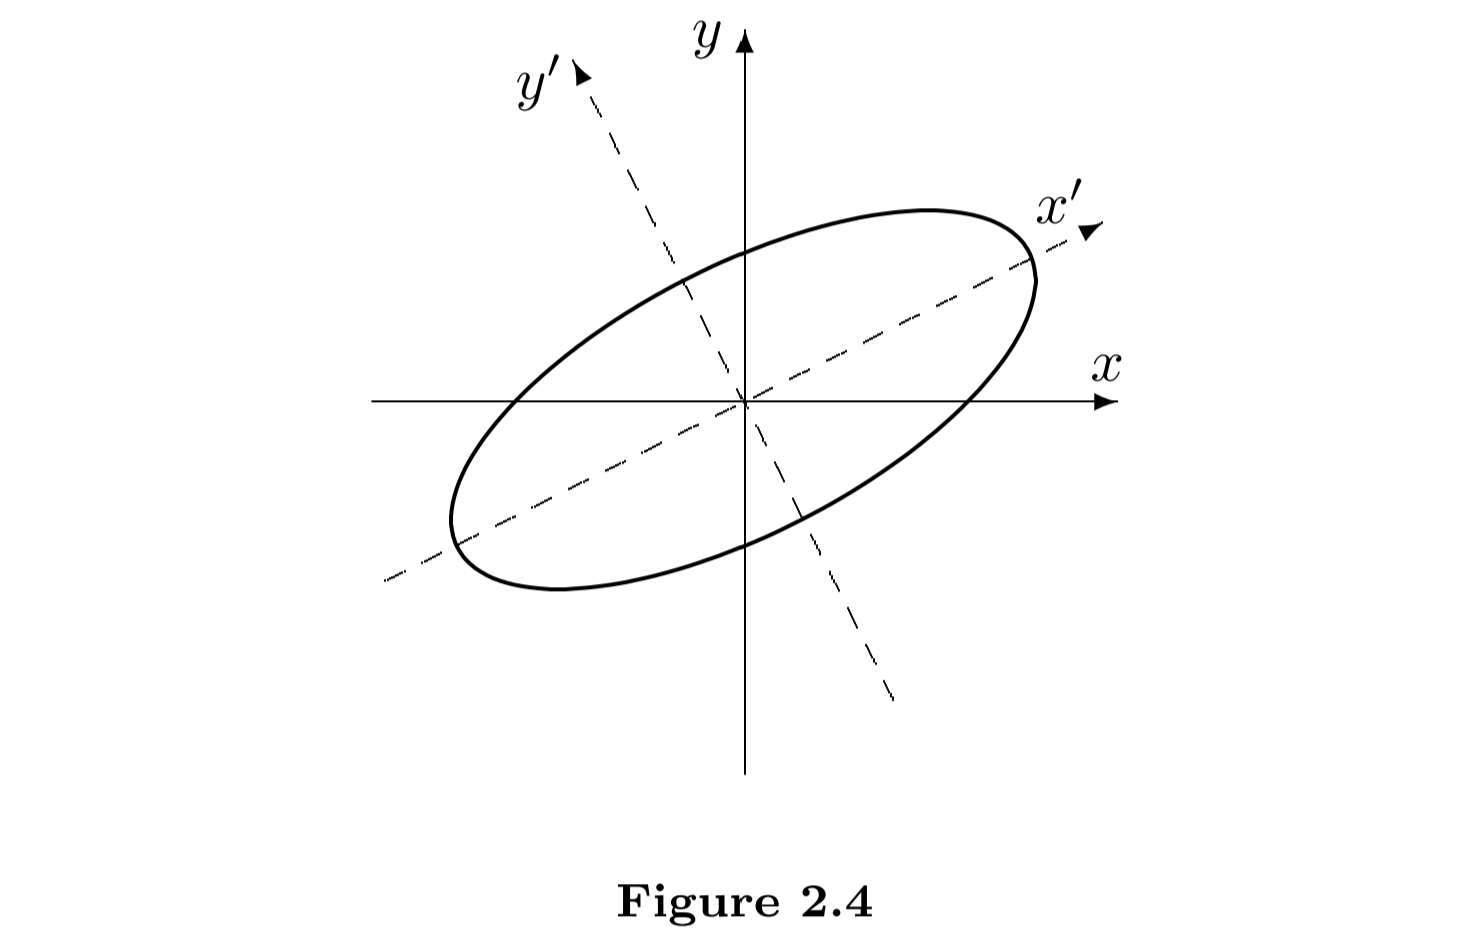
\includegraphics[width=10cm]{images/figure-2-4.png}

We will see how this change of variable is \emph{determined} in \SEC{6.5}.

(For figure 2.4,) Geometrically, the change of variable
\[
    P = \begin{pmatrix} x \\ y \end{pmatrix} \to \begin{pmatrix} x' \\ y' \end{pmatrix}
\]
is a \emph{change in the way} that the position of a point \(P\) in the plane is \emph{described}.
This is done by \emph{introducing a new frame of reference}, an \(x'y'\)-coordinate system with coordinate axes \emph{rotated} from the original \(xy\)-coordinate axes.
In this case, the new coordinate axes(\(x'\)-axis and \(y'\)-axis) are chosen to \emph{lie in the direction of the axes} of the ellipse.
The \textbf{unit vectors} along the \(x'\)-axis and the \(y'\)-axis form an \emph{ordered basis} for \(\SET{R}^2\):
\[
    \beta' = \bigg\{ \frac{1}{\sqrt{5}} \begin{pmatrix} 2 \\ 1 \end{pmatrix}, \frac{1}{\sqrt{5}} \begin{pmatrix} -1 \\ 2 \end{pmatrix} \bigg\}
\]
and the change of variable is actually a change from \([P]_{\beta} = \begin{pmatrix} x \\ y \end{pmatrix}\), the coordinate vector of \(P\) relative to the \emph{standard} ordered basis \(\beta = \{ e_1, e_2 \}\), to \([P]_{\beta'} = \begin{pmatrix} x' \\ y' \end{pmatrix}\), the coordinate vector of \(P\) relative to the new rotated basis \(\beta'\).

A natural question arises:
How can a coordinate vector relative to one basis be changed into a coordinate vector relative to the other?
Notice that the \emph{system of equations} relating the new and old coordinates can be represented by the matrix equation
\[
    \begin{pmatrix} x \\ y \end{pmatrix}
    = \frac{1}{\sqrt{5}} \begin{pmatrix}
        2 & -1 \\ 1 & 2
    \end{pmatrix} \begin{pmatrix} x' \\ y' \end{pmatrix}.
\]
Notice also that
\[
    Q = \frac{1}{\sqrt{5}} \begin{pmatrix}
        2 & -1 \\ 1 & 2
    \end{pmatrix}
\]
equals \([\mathrm{I}]_{\beta'}^{\beta}\), where \(\mathrm{I}\) denotes the \emph{identity transformation} on \(\SET{R}^2\).
Thus \([v]_{\beta} = Q[v]_{\beta'}\) for all \(v \in \SET{R}^2\).
(Also notice the \textbf{order} of the bases of the matrix representation;
the matrix representation is from the basis we want to change into the basis we originally have.)
A similar result is true in general.

\begin{theorem} \label{thm 2.22}
Let \(\beta\) and \(\beta'\) be two ordered bases for a finite-dimensional vector space \(V\), and let \(Q = [\ITRANV]_{\beta'}^{\beta}\).
Then
\begin{enumerate}
\item \(Q\) is invertible.
\item For any \(v \in V\), \([v]_{\beta} = Q[v]_{\beta'}\).
\end{enumerate}
\end{theorem}

\begin{proof} \ 

\begin{enumerate}
\item Since \(\ITRANV\) is invertible, \(Q\) is invertible by \THM{2.18}.

\item For any \(v \in V\),
\begin{align*}
    [v]_{\beta} & = [\ITRANV(v)]_{\beta} & \text{of course} \\
                & = [\ITRANV]_{\beta'}^{\beta} [v]_{\beta'} & \text{by \THM{2.14}} \\
                & = Q [v]_{\beta'}.
\end{align*}
\end{enumerate}
\end{proof}

\begin{remark} \label{remark 2.5.1}
The matrix \(Q = [\ITRANV]_{\beta'}^{\beta}\), defined in \THM{2.22}, is called \textbf{a change of coordinate matrix}.
Because of part (b) of the theorem, we say that \textbf{\(Q\) changes \(\beta'\)-coordinates into \(\beta\)-coordinates}.
Observe that if \(\beta = \{ x_1, x_2, ..., x_n \}\) and \(\beta' = \{ x'_1, x'_2, ..., x'_n \}\), then by definition of matrix representation, the \(j\)th column of \(Q = [\ITRANV]_{\beta'}^{\beta}\) is \([\ITRANV(x'_j)]_{\beta}\).
But since \([\ITRANV(x'_j)]_{\beta} = [x'_j]_{\beta}\), the \(j\)th column of \(Q\) is \([x'_j]_{\beta}\).
\end{remark}

\begin{note}
上面那段\ remark 是想表達,給定一個從原座標\ \(\beta'\) 轉換到目標座標\ \(\beta\) 的轉換矩陣,該矩陣的第\ \(j\) 行就是原座標\ \(\beta'\) 的第\ \(j\) 個\ vector,在用目標座標\ \(\beta\) 來表示時的座標向量。
\end{note}

Also notice that if \(Q\) changes \(\beta'\)-coordinates into \(\beta\)-coordinates, then \(Q^{-1}\) changes \(\beta\)-coordinates into \(\beta'\)-coordinates. (See \EXEC{2.5.11}.)

\begin{example} \label{example 2.5.1}
In \(\SET{R}^2\), let \(\beta = \{ (1, 1), (1, -1) \}\) and \(\beta' = \{ (2, 4), (3, 1) \}\).
Since
\[
    (2, 4) = 3(1, 1) - 1(1, - 1) \text{ and } (3, 1) = 2(1, 1) + 1(1, -1),
\]
The matrix that changes \(\beta\)'-coordinates into \(\beta\)-coordinates is
\[
    Q = \begin{pmatrix} 3 & 2 \\ -1 & 1 \end{pmatrix}.
\]
Thus, for instance, given a \emph{(normal) vector} \((2, 4) \in \SET{R}^2\),
\begin{align*}
    [(2, 4)]_{\beta} & = Q[(2, 4)]_{\beta'} & \text{by \THM{2.22}} \\
                     & = Q \begin{pmatrix} 1 \\ 0 \end{pmatrix} & \text{since \((2, 4)\) is the first vector of \(\beta'\)} \\
                     & = \begin{pmatrix} 3 \\ -1 \end{pmatrix} & \text{by calculation}
\end{align*}
\end{example}

\begin{note}
\((2, 4)\) in this example is \textbf{not} considered to be a coordinate vector; it simply is a ``normal'' vector of \(\SET{R}^2\).
However, \(\begin{pmatrix} 3 \\ -1 \end{pmatrix}\) is a coordinate vector;
if we consider a vector to be a coordinate vector, we write its components vertically, or horizontally but adding transpose to it.
\end{note}

For the remainder of this section, we consider only \LTRAN{}s that map a vector space \(V\) \emph{into itself}.
Such a \LTRAN{} is called a \textbf{linear operator} on \(V\).
(I have defined the term in \DEF{2.1}.)

Now suppose now that \(\T\) is a linear operator on a finite-dimensional vector space \(V\) and that \(\beta\) and \(\beta'\) are ordered bases for \(V\).
Then \(V\) can be represented by the matrices \([\T]_{\beta}\) and \([\T]_{\beta'}\).
What is the \emph{relationship} between these matrices?
The next theorem provides a simple answer using a
change of coordinate matrix.

\begin{theorem} \label{thm 2.23}
Let \(\T\) be a linear operator on a finite-dimensional vector space \(V\),
and let \(\beta\) and \(\beta'\) be ordered bases for \(V\).
Suppose that \(Q\) is the change of coordinate matrix that changes \(\beta'\)-coordinates into \(\beta\)-coordinates.
Then
\[
    [\T]_{\beta} = Q^{-1} [\T]_{\beta'} Q.
\]
\end{theorem}

\begin{note}
Related exercise: \EXEC{2.4.16}.
\end{note}

\begin{proof}
Let \(\ITRANV\) be the identity transformation on \(V\).
Then
\begin{align*}
    Q [\T]_{\beta'} & = [\ITRANV]_{\beta'}^{\beta} [\T]_{\beta'} & \text{by def of \(Q\)} \\
                    & = [\ITRANV \T]_{\beta'}^{\beta} & \text{by \THM{2.11}} \\
                    & = [\T \ITRANV]_{\beta'}^{\beta} & \text{by \THM{2.10}(c)} \\
                    & = [\T]_{\beta} [\ITRANV]_{\beta'}^{\beta} & \text{by \THM{2.11}} \\
                    & = [\T]_{\beta} Q & \text{by def of \(Q\)}
\end{align*}
which implies
\begin{align*}
             & Q [\T]_{\beta'} = [\T]_{\beta} Q \\
    \implies & Q^{-1} Q [\T]_{\beta'} = Q^{-1} [\T]_{\beta} Q & \text{by multiplying \(Q^{-1}\) on the left} \\
    \implies & [\T]_{\beta'} = Q^{-1} [\T]_{\beta} Q. & \text{of course}
\end{align*}
\end{proof}

\begin{example} \label{example 2.5.2}
Let \(\T\) be the linear operator on \(\SET{R}^2\) defined by
\[
    \T \begin{pmatrix} a \\ b \end{pmatrix} = \begin{pmatrix} 3a - b \\ a + 3b \end{pmatrix}
\]
let \(\beta = \{ (1, 1), (1, -1) \}\) and \(\beta' = \{ (2, 4), (3, 1) \}\).
The reader should verify that
\[
    [\T]_{\beta} = \begin{pmatrix} 3 & 1 \\ -1 & 3 \end{pmatrix}
\]
In \EXAMPLE{2.5.1}, we saw that the change of coordinate matrix that changes \(\beta'\)-coordinates into \(\beta\)-coordinates is
\[
    Q = \begin{pmatrix} 3 & 2 \\ -1 & 1 \end{pmatrix}.
\]
and it is easily verified that
\[
    Q^{-1} = \frac{1}{5} \begin{pmatrix} 1 & -2 \\ 1 & 3 \end{pmatrix}.
\]
Hence, by \THM{2.23},
\[
    [\T]_{\beta'} = Q^{-1} [\T]_{\beta} Q = \begin{pmatrix} 4 & 1 \\ -2 & -2 \end{pmatrix}.
\]
To show that this \([\T]_{\beta'}\) is really the correct matrix, we can verify that the image under \(\T\) of each vector of \(\beta'\) is the linear combination of the vectors of \(\beta'\) with the entries of the corresponding column as this \([\T]_{\beta'}\)'s coefficients.
For example, the image of the \emph{second} vector in \(\beta'\) is
\[
    \T \begin{pmatrix} 3 & 1 \end{pmatrix} = \begin{pmatrix} 8 & 6 \end{pmatrix} = \RED{1} \begin{pmatrix} 2 & 4 \end{pmatrix} + \RED{3} \begin{pmatrix} 3 & 1 \end{pmatrix}
\]
Notice that the coefficients of the linear combination are the entries of the \emph{second} column of this \([\T]_{\beta'}\).
\end{example}

\begin{note}
It is often useful to apply \THM{2.23} to compute \([\T]_{\beta}\), as the next example shows.
\end{note}

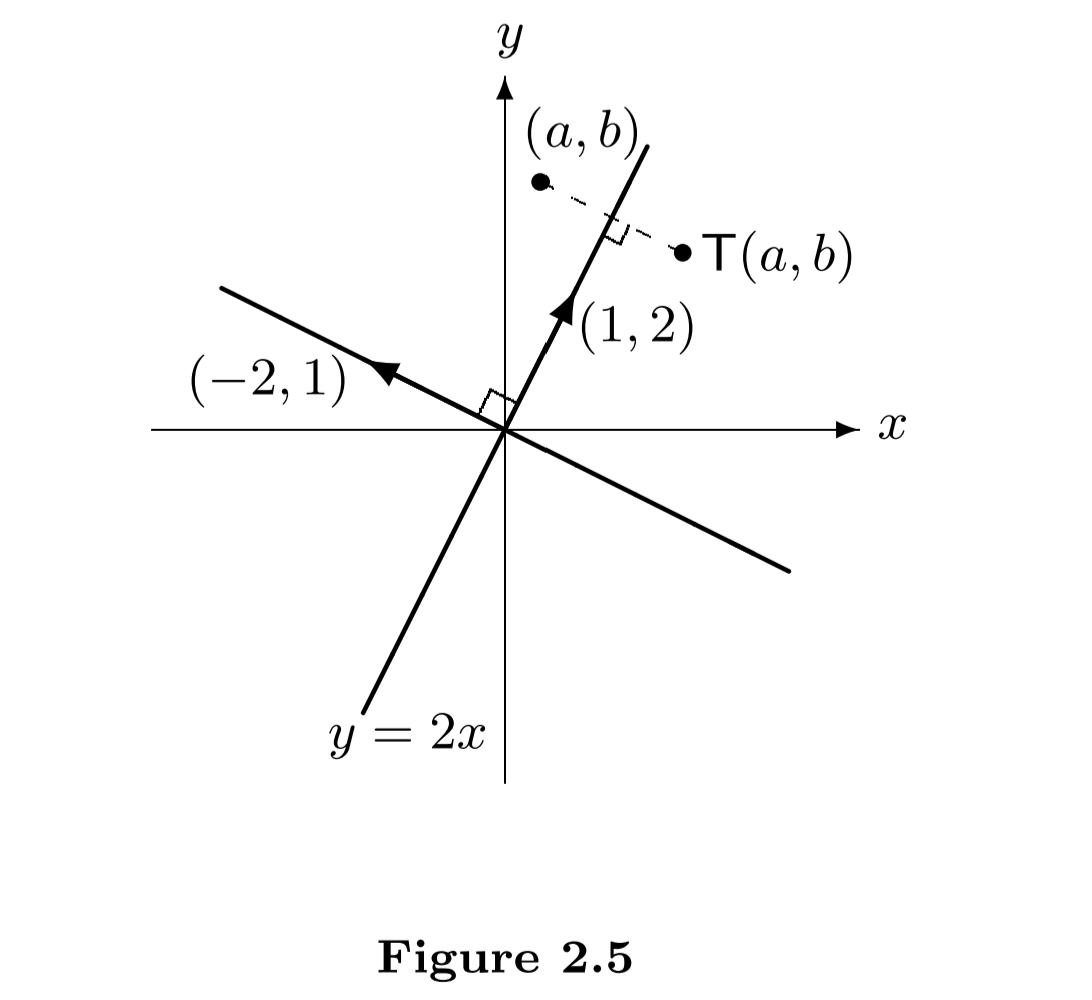
\includegraphics[width=8cm]{images/figure-2-5.png}

\begin{example} \label{example 2.5.3}
Recall the \emph{reflection} about the \(x\)-axis in \EXAMPLE{2.1.3}.
The rule \((x, y) \to (x, -y)\) is easy to obtain.
We now derive the less obvious rule for the \emph{reflection} \(\T\) \emph{about the line} \(y = 2x\). (See Figure 2.5.)

We wish to find \emph{an expression} for \(\T(a,b)\) for any \((a,b) \in \SET{R}^2\).
Since \(\T\) is linear, (by \THM{2.6}) it is completely
determined by its values on \emph{a basis} for \(\SET{R}^2\).
Clearly, from figure 2.5 we have \(\T(1, 2) = (1, 2) = 1 \cdot (1, 2) + 0 \cdot (-2, 1)\) and \(\T(-2, 1) = -(-2, 1) = 0 \cdot (1, 2) + (-1) \cdot (-2, 1)\), where \(\{ (1, 2), (-2, 1) \}\) is a basis for \(\SET{R}^2\).
Then we let \(\beta' = \{ (1, 2), (-2, 1) \}\), from these result (and \THM{2.6}),
\[
    [\T]_{\beta'} = \begin{pmatrix} 1 & 0 \\ 0 & -1 \end{pmatrix}.
\]

Now let \(\beta\) be the \emph{standard} ordered basis for \(\SET{R}^2\), and let \(Q\) be the matrix that changes \(\beta'\)-coordinates into \(\beta\)-coordinates.

Then (by calculation),
\[
    Q = \begin{pmatrix} 1 & -2 \\ 2 & 1 \end{pmatrix}
\]
And from \THM{2.23} and some calculation(see \EXEC{2.5.1}(c)) we have \([\T]_{\beta} = Q[\T]_{\beta'}Q^{-1}\).
Because (mysteriously)
\[
    Q^{-1} = \frac{1}{5} \begin{pmatrix} 1 & 2 \\ -2 & 1 \end{pmatrix}
\]
the reader can verify that
\[
    [\T]_{\beta} = \frac{1}{5} \begin{pmatrix} -3 & 4 \\ 4 & 3 \end{pmatrix}
\]
Since \(\beta\) is the standard ordered basis, it follows by \THM{2.15}(a) that \(\T\) is left-multiplication by \([\T]_{\beta}\).
Thus for any \((a, b) \in \SET{R}^2\), we have
\[
    \T \begin{pmatrix} a \\ b \end{pmatrix}
    = \frac{1}{5} \begin{pmatrix} -3 & 4 \\ 4 & 3 \end{pmatrix} \begin{pmatrix} a \\ b \end{pmatrix}
    = \frac{1}{5} \begin{pmatrix} -3a + 4b \\ 4a + 3b \end{pmatrix}.
\]
\end{example}

A useful special case of \THM{2.23} is contained in the next corollary.

\begin{corollary} \label{corollary 2.23.1}
Let \(A \in M_{n \X n}(F)\), and let \(\gamma\) be an ordered basis for \(F^n\).
Then \([\LMTRAN_A]_{\gamma} = Q^{-1} A Q\), where \(Q\) is the \(n \X n\) matrix whose \(j\)th column is the \(j\)th vector of \(\gamma\).
\end{corollary}

\begin{proof}
Let \(\beta\) be the \emph{standard} ordered basis for \(F^n\), then by \THM{2.15}(a), \([\LMTRAN_A]_{\beta} = A\).
Then by \THM{2.23}, \([\LMTRAN_A]_{\gamma} = Q^{-1} [\LMTRAN_A]_{\beta} Q\) where \(Q\) is the coordinate matrix that changes \(\gamma\)-coordinates into \(\beta\)-coordinates.
And from \RMK{2.5.1}, the \(j\)th column of \(Q\) is \([v_j]_{\beta}\) where \(v_j\) is the \(j\)th vector of \(\gamma\).
But since \(\beta\) is standard ordred basis, we have \([v_j]_{\beta} = v_j\), so the \(j\)th column of \(Q\) is \(v_j\), as desired.
\end{proof}

\begin{note}
這個\ corollary 是\ \RMK{2.5.1} 的「更加\ special case」:
當我們把某個基底座標\textbf{轉換成標準基底座標},則那個座標轉換矩陣的第\ \(j\) 行就直接等於那個基底座標的第\ \(j\) 個向量。
\end{note}

\begin{example} \label{example 2.5.4}
Let
\[
    A = \begin{pmatrix}
        2 & 1 & 0 \\ 1 & 1 & 3 \\ 0 & -1 & 0
    \end{pmatrix},
\]
and let
\[
    \gamma = \bigg\{
        \begin{pmatrix} -1 \\ 0 \\ 0 \end{pmatrix}, 
        \begin{pmatrix} 2 \\ 1 \\ 0 \end{pmatrix}, 
        \begin{pmatrix} 1 \\ 1 \\ 1 \end{pmatrix}
    \bigg\},
\]
which is an ordered basis for \(\SET{R}^3\).
Let \(Q\) be the \(3 \X 3\) matrix whose \(j\)th column is the \(j\)th vector of \(\gamma\). (this satisfies the condition of \CORO{2.23.1}.)
Then
\[
    Q = \begin{pmatrix} -1 & 2 & 1 \\ 0 & 1 & 1 \\ 0 & 0 & 1 \end{pmatrix}
    \text{ and (mysteriously) }
    Q^{-1} = \begin{pmatrix} -1 & 2 & -1 \\ 0 & 1 & -1 \\ 0 & 0 & 1 \end{pmatrix}.
\]
So by \CORO{2.23.1},
\[
    [\LMTRAN_A]_{\gamma} = Q^{-1} A Q = \begin{pmatrix} 0 & 2 & 8 \\ -1 & 4 & 6 \\ 0 & -1 & -1 \end{pmatrix}.
\]
\end{example}

\begin{remark} \label{remark 2.5.2}
The relationship, defined immediately, between the matrices \([\T]_{\beta'}\) and \([\T]_{\beta}\) in \THM{2.23} \textbf{will be the subject of further study in \CH{5}, \CH{6}, and \CH{7}}.
\end{remark}

\begin{definition} \label{def 2.16}
Let \(A\) and \(B\) be matrices in \(M_{n \X n}(F)\).
We say that \(B\) is \textbf{similar}\textbf{} to \(A\) if there exists an \textbf{invertible matrix} \(Q\) such that \(B = Q^{-1} A Q\).
\end{definition}

\begin{remark} \label{remark 2.5.3}
Observe that the relation of similarity is an \textbf{equivalence relation} (see \EXEC{2.5.9}).
So we need only say that \(A\) and \(B\) are similar.

Notice also that in this terminology \THM{2.23} can be stated as follows:
If \(\T\) is a linear operator on a finite-dimensional vector space \(V\), and if \(\beta\) and \(\beta'\) are any ordered bases for \(V\), then \([\T]_{\beta'}\) is similar to \([\T]_{\beta}\).
\end{remark}

\begin{remark} \label{remark 2.5.4}
\THM{2.23} can be \emph{generalized} to allow \(\T : V \to W\), where \(V\) is distinct from \(W\).
In this case, we can change bases in \(V\) as well as in \(W\) (see \EXEC{2.5.8}).
\end{remark}

\exercisesection

\begin{exercise} \label{exercise 2.5.1}
Label the following statements as true or false.
\begin{enumerate}
\item Suppose that \(\beta = \{ x_1, x_2, ..., x_n \}\) and \(\beta' = \{ x'_1, x'_2, ..., x'_n \}\) are ordered bases for a vector space
and \(Q\) is the change of coordinate matrix that changes \(\beta'\)-coordinates into \(\beta\)-coordinates.
Then the \(j\)th column of \(Q\) is \([x_j]_{\beta'}\).

\item Every change of coordinate matrix is invertible. 

\item Let \(\T\) be a linear operator on a finite-dimensional vector space \(V\), let \(\beta\) and \(\beta'\) be ordered bases for \(V\),
and let \(Q\) be the change of coordinate matrix that changes \(\beta'\)-coordinates into \(\beta\)-coordinates.
Then \([\T]_{\beta} = Q [\T]_{\beta'} Q^{-1}\).

\item The matrices \(A, B \in M_{n \X n}(F)\) are called similar if \(B = Q^\top A Q\) for some \(Q \in M_{n \X n}(F)\).

\item Let \(\T\) be a linear operator on a finite-dimensional vector space \(V\).
Then for any ordered bases \(\beta\) and \(\gamma\) for \(V\), \([\T]_{\beta}\) is similar to \([\T]_{\gamma}\).
\end{enumerate}
\end{exercise}

\begin{proof} \ 

\begin{enumerate}
\item False. By \RMK{2.5.1}, the \(j\)th column of \(Q\) is \([x'_j]_{\beta}\).
\item True by \THM{2.22}(a).
\item True.
    We have
    \begin{align*}
                 & [\T]_{\beta'} = Q^{-1}[\T]_{\beta}Q & \text{by \THM{2.23}} \\
        \implies & Q [\T]_{\beta'} Q^{-1} = Q (Q^{-1} [\T]_{\beta} Q) Q^{-1} & \text{by multiplying \(Q\) in the left and \(Q^{-1}\) in the right} \\
        \implies & Q [\T]_{\beta'} Q^{-1} = [\T]_{\beta},
    \end{align*}
    as desired.
\item False by \DEF{2.16}.
\item True by \RMK{2.5.3}.
\end{enumerate}
\end{proof}

\begin{exercise} \label{exercise 2.5.2}
For each of the following pairs of ordered bases \(\beta\) and \(\beta'\) for \(\SET{R}^2\), find the change of coordinate matrix that changes \(\beta'\)-coordinates into \(\beta\)-coordinates.
\begin{enumerate}
\item \(\beta = \{ e_1, e_2 \}\) and \(\beta' = \{ (a_1, a_2), (b_1, b_2) \}\).
\item \(\beta = \{ (-1, 3), (2, -1) \}\) and \(\beta' = \{ (0, 10), (5, 0) \}\).
\item \(\beta = \{ (2, 5), (-1, -3) \}\) and \(\beta' = \{ e_1, e_2 \}\).
\item \(\beta = \{ (-4, 3), (2, -1) \}\) and \(\beta' = \{ (2, 1), (-4, 1) \}\).
\end{enumerate}
\end{exercise}

\begin{proof} \ 

\begin{enumerate}
\item We have \((a_1, a_2) = a_1 \cdot e_1 + a_2 \cdot e_2\), \((b_1, b_2) = b_1 \cdot e_1 + b_2 \cdot e_2\), so
\[ Q = \begin{pmatrix} a_1 & b_1 \\ a_2 & b_2 \end{pmatrix}. \]

\item (By solving system of equations), \((0, 10) = 4 \cdot (-1, 3) + 2 \cdot (2, -1)\), \((5, 0) = 1 \cdot (-1, 3) + 3 \cdot (2, -1)\), so
\[ Q = \begin{pmatrix} 4 & 1 \\ 2 & 3 \end{pmatrix}. \]

\item (By solving system of equations), \(e_1 = 3 \cdot (2, 5) + 5 \cdot (-1, -3)\), \(e_2 = -1 \cdot (2, 5) + (-2) \cdot (-1, -3)\), so
\[ Q = \begin{pmatrix} 3 & -1 \\ 5 & -2 \end{pmatrix}. \]

\item (By solving system of equations), \((2, 1) = 2 \cdot (-4, 3) + 5 \cdot (2, -1)\), \((-4, 1) = -1 \cdot (-4, 3) + (-4) \cdot (2, -1)\), so
\[ Q = \begin{pmatrix} 2 & -1 \\ 5 & -4 \end{pmatrix}. \]
\end{enumerate}
\end{proof}

\begin{exercise} \label{exercise 2.5.3}
Skip, tedious.
\end{exercise}

\begin{exercise} \label{exercise 2.5.4}
Let \(\T\) be the linear operator on \(\SET{R}^2\) defined by
\[
    \T\begin{pmatrix} a \\ b \end{pmatrix}
    = \begin{pmatrix} 2a + b \\ a - 3b \end{pmatrix},
\]
let \(\beta\) be the standard ordered basis for \(\SET{R}^2\), and let
\[
    \beta' = \bigg\{ \begin{pmatrix} 1 \\ 1 \end{pmatrix},
    \begin{pmatrix} 1 \\ 2 \end{pmatrix} \bigg\}.
\]
Use \THM{2.23} and the (mysterious) fact that
\[
    \begin{pmatrix} 1 & 1 \\ 1 & 2 \end{pmatrix}^{-1} =
    \begin{pmatrix} 2 & -1 \\ -1 & 1 \end{pmatrix}
\]
to find \([\T]_{\beta'}\).
\end{exercise}

\begin{proof}
First \([\T]_{\beta} = \begin{pmatrix} 2 & 1 \\ 1 & -3 \end{pmatrix}\), since \(\T(e_1) = \begin{pmatrix} 2 \\ 1 \end{pmatrix}= 2 \cdot e_1 + 1 \cdot e_2\) and \(\T(e_2) = \begin{pmatrix} 1 \\ -3 \end{pmatrix} = 1 \cdot e_1 + (-3) \cdot e_2\).
And by solving equation we know \(Q = \begin{pmatrix} 1 & 1 \\ 1 & 2 \end{pmatrix}\).
Then by \THM{2.23} and the provided fact,
\[
    [\T]_{\beta'} = Q^{-1} [\T]_{\beta} Q =
    \begin{pmatrix} 2 & -1 \\ -1 & 1 \end{pmatrix}
    \begin{pmatrix} 2 & 1 \\ 1 & -3 \end{pmatrix}
    \begin{pmatrix} 1 & 1 \\ 1 & 2 \end{pmatrix}
    = \begin{pmatrix} 8 & 13 \\ -5 & -9 \end{pmatrix}
\]
\end{proof}

\begin{exercise} \label{exercise 2.5.5}
Let \(\T\) be the linear operator on \(\mathcal{P}_1(\SET{R})\) defined by \(\T(p(x)) = p'(x)\), the derivative of \(p(x)\).\
Let \(\beta = \{ 1, x \}\) and \(\beta' = \{ 1 + x, 1 - x \}\).
Use \THM{2.23} and the fact that
\[
    \begin{pmatrix} 1 & 1 \\ 1 & -1 \end{pmatrix}^{-1} =
    \begin{pmatrix} \frac1{2} & \frac1{2} \\ \frac1{2} & -\frac1{2} \end{pmatrix}
\]
to find \([\T]_{\beta'}\).
\end{exercise}

\begin{proof}

First \([\T]_{\beta} = \begin{pmatrix} 0 & 1 \\ 0 & 0 \end{pmatrix}\) since \(\T(1) = 0 = 0 \cdot 1 + 0 \cdot x\) and \(\T(x) = 1 = 1 \cdot 1 + 0 \cdot x\).
And by solving equation we know \(Q = \begin{pmatrix} 1 & 1 \\ 1 & -1 \end{pmatrix}\).
Then by \THM{2.23} and the provided fact,
\[
    [\T]_{\beta'} = Q^{-1} [\T]_{\beta} Q =
    \begin{pmatrix} \frac1{2} & \frac1{2} \\ \frac1{2} & -\frac1{2} \end{pmatrix}
    \begin{pmatrix} 0 & 1 \\ 0 & 0 \end{pmatrix}
    \begin{pmatrix} 1 & 1 \\ 1 & -1 \end{pmatrix}
    = \begin{pmatrix} \frac1{2} & -\frac1{2} \\ \frac1{2} & -\frac1{2} \end{pmatrix}
\]
\end{proof}

\begin{exercise} \label{exercise 2.5.6}
For each matrix \(A\) and ordered basis \(\beta\), find \([\LMTRAN_A]_{\beta}\).
Also, find an invertible matrix \(Q\) such that \([\LMTRAN_A]_{\beta} = Q^{-1} A Q\).

\begin{enumerate}
\item \(A = \begin{pmatrix} 1 & 3 \\ 1 & 1 \end{pmatrix}\) and \(\beta = \bigg\{
    \begin{pmatrix} 1 \\ 1 \end{pmatrix},
    \begin{pmatrix} 1 \\ 2 \end{pmatrix}
\bigg\}\)

\item \(A = \begin{pmatrix} 1 & 2 \\ 2 & 1 \end{pmatrix}\) and \(\beta = \bigg\{
    \begin{pmatrix} 1 \\ 1 \end{pmatrix},
    \begin{pmatrix} 1 \\ -1 \end{pmatrix}
\bigg\}\)

\item \(A = \begin{pmatrix} 1 & 1 & -1 \\ 2 & 0 & 1 \\ 1 & 1 & 0 \end{pmatrix}\) and \(\beta = \bigg\{
    \begin{pmatrix} 1 \\ 1 \\ 1 \end{pmatrix},
    \begin{pmatrix} 1 \\ 0 \\ 1 \end{pmatrix},
    \begin{pmatrix} 1 \\ 1 \\ 2 \end{pmatrix}
\bigg\}\)

\item \(A = \begin{pmatrix} 13 & 1 & 4 \\ 1 & 13 & 4 \\ 4 & 4 & 10 \end{pmatrix}\) and \(\beta = \bigg\{
    \begin{pmatrix} 1 \\ 1 \\ -2 \end{pmatrix},
    \begin{pmatrix} 1 \\ -1 \\ 0 \end{pmatrix},
    \begin{pmatrix} 1 \\ 1 \\ 1 \end{pmatrix}
\bigg\}\)
\end{enumerate}
\end{exercise}

\begin{proof}
From \CORO{2.23.1}, \([\LMTRAN_A]_{\beta} = Q^{-1} A Q\), where \(Q\) is the \(n \X n\) matrix whose \(j\)th column is the \(j\)th vector of \(\beta\).
Hence

\begin{enumerate}
\item \(Q = \begin{pmatrix} 1 & 1 \\ 1 & 2 \end{pmatrix}\).

\item \(Q = \begin{pmatrix} 1 & 1 \\ 1 & -1 \end{pmatrix}\).

\item \(Q = \begin{pmatrix} 1 & 1 & 1 \\ 1 & 0 & 1 \\ 1 & 1 & 2 \end{pmatrix}\).

\item \(Q = \begin{pmatrix} 1 & 1 & 1 \\ 1 & -1 & 1 \\ -2 & 0 & 1 \end{pmatrix}\).
\end{enumerate}

I skip computing \([\LMTRAN_A]_{\beta}\), since either computing it directly or using \CORO{2.23.1} but requiring \(Q^{-1}\) are tedious.
\end{proof}

\begin{exercise} \label{exercise 2.5.7}
In \(\SET{R}^2\), let \(L\) be the line \(y = mx\), where \(m \ne 0\).
Find an expression for \(\T(x, y)\), where
\begin{enumerate}
\item \(\T\) is the reflection of \(\SET{R}^2\) about \(L\).
\item \(\T\) is the projection(see \ADEF{2.2}) on \(L\) along the line \emph{perpendicular} to \(L\).
\end{enumerate}
\end{exercise}

\begin{proof}
We may let \(\beta\) be the standard ordered basis and \(\alpha = \{ (1, m), (-m, 1) \}\) be another basis for \(\SET{R}^2\).
\begin{enumerate}
\item We have that \([\T]_{\alpha} = \begin{pmatrix} 1 & 0 \\ 0 & -1 \end{pmatrix}\) and (by \EXEC{2.5.11}) \(Q^{-1} = [\mathrm{I}]_{\alpha}^{\beta} = \begin{pmatrix} 1 & m \\ -m & 1 \end{pmatrix}\).
We can also calculate that \(Q = [\mathrm{I}]_{\beta}^{\alpha} = \begin{pmatrix} \frac{1}{m^2 + 1} & \frac{m}{m^2 + 1} \\ -\frac{m}{m^2 + 1} & \frac{1}{m^2 + 1} \end{pmatrix}\).
So by \THM{2.23}, we have
\[
    [\T]_{\beta} = Q^{-1} [\T]_{\alpha} Q = \begin{pmatrix}
        \frac{1 - m^2}{m^2 + 1} & \frac{2m}{m^2 + 1} \\
        \frac{2m}{m^2 + 1} & \frac{m^2 - 1}{m^2 + 1}
    \end{pmatrix}.
\]
And we have
\begin{align*}
    & \T \begin{pmatrix} x \\ y \end{pmatrix} \\
    & = \left[ \T \begin{pmatrix} x \\ y \end{pmatrix} \right]_{\beta} & \text{since domain/codomain are actually \(\SET{R}^n\) and \(\beta\) is standard} \\
    & = [\T]_{\beta} \left[ \begin{pmatrix} x \\ y \end{pmatrix} \right]_{\beta} & \text{by \THM{2.14}} \\
    & = [\T]_{\beta} \begin{pmatrix} x \\ y \end{pmatrix} & \text{since domain/codomain are actually \(\SET{R}^n\) and \(\beta\) is standard} \\
    & = \begin{pmatrix}
            \frac{1 - m^2}{m^2 + 1} & \frac{2m}{m^2 + 1} \\
            \frac{2m}{m^2 + 1} & \frac{m^2 - 1}{m^2 + 1}
        \end{pmatrix}
        \begin{pmatrix} x \\ y \end{pmatrix} \\
    & = \begin{pmatrix}
            \frac{x-m^{2} x+2 m y}{1+m^{2}} \\
            \frac{2 m x+m^{2} y-y}{1+m^{2}}
        \end{pmatrix}
\end{align*}

\item Similarly we have that \([\T]_{\alpha} = \begin{pmatrix} 1 & 0 \\ 0 & 0 \end{pmatrix}\).
And with the same \(Q^{-1}\) and \(Q\) we have
\[
    [\T]_{\beta} = Q^{-1} [\T]_{\alpha} Q = \begin{pmatrix}
        \frac{1}{m^2 + 1} & \frac{m}{m^2 + 1} \\
        \frac{m}{m^2 + 1} & \frac{m^2}{m^2 + 1}
    \end{pmatrix}.
\]
So 
\begin{align*}
    & \T \begin{pmatrix} x \\ y \end{pmatrix} \\
    & = [\T]_{\beta} \begin{pmatrix} x \\ y \end{pmatrix} & \text{similar derivation from part(a)} \\
    & = \begin{pmatrix}
            \frac{1}{m^2 + 1} & \frac{m}{m^2 + 1} \\
            \frac{m}{m^2 + 1} & \frac{m^2}{m^2 + 1}
        \end{pmatrix}
        \begin{pmatrix} x \\ y \end{pmatrix} \\
    & = \begin{pmatrix}
            \frac{x + ym}{m^{2} + 1} \\
            \frac{xm + ym^2}{m^{2} + 1}
        \end{pmatrix}
\end{align*}

\end{enumerate}
\end{proof}

\begin{exercise} \label{exercise 2.5.8}
Prove the following \emph{generalization} of \THM{2.23}.
Let \(\T : V \to W\) be a \LTRAN{} from a finite-dimensional vector space \(V\) to a finite-dimensional vector space \(W\).
Let \(\beta\) and \(\beta'\) be ordered bases for \(V\), and let \(\gamma\) and \(\gamma'\) be ordered bases for \(W\).
Then \([\T]_{\beta'}^{\gamma'} = P^{-1} [\T]_{\beta}^{\gamma} Q\), where \(Q\) is the matrix that changes \(\beta'\)-coordinates into \(\beta\)-coordinates and \(P\) is the matrix that changes \(\gamma'\)-coordinates into \(\gamma\)-coordinates.
\end{exercise}

\begin{proof}
By (the generalization of) \THM{2.10}(c), we have \(\T = \ITRANW \T = \T \ITRANV\) \MAROON{(1)}.

Then we have
\begin{align*}
    P [\T]_{\beta'}^{\gamma'}
        & = [\ITRANW]_{\gamma'}^{\gamma} [\T]_{\beta'}^{\gamma'} & \text{by def of \(P\)} \\
        & = [\ITRANW\T]_{\beta'}^{\gamma} & \text{by \THM{2.11}} \\
        & = [\T\ITRANV]_{\beta'}^{\gamma} & \text{by \MAROON{(1)}} \\
        & = [\T]_{\beta}^{\gamma} [\ITRANV]_{\beta'}^{\beta} & \text{\THM{2.11}} \\
        & = [\T]_{\beta}^{\gamma} Q & \text{by def of \(Q\)}
\end{align*}
So we have \(P [\T]_{\beta'}^{\gamma'} = [\T]_{\beta}^{\gamma} Q\).
And
\begin{align*}
             & P [\T]_{\beta'}^{\gamma'} = [\T]_{\beta}^{\gamma} Q \\
    \implies & P^{-1} P [\T]_{\beta'}^{\gamma'} = P^{-1} [\T]_{\beta}^{\gamma} Q & \text{by multiplying \(P^{-1}\) in the left} \\
    \implies & [\T]_{\beta'}^{\gamma'} = P^{-1} [\T]_{\beta}^{\gamma} Q, & \text{of course}
\end{align*}
as desired.
\end{proof}

\begin{exercise} \label{exercise 2.5.9}
Prove that "is similar to" is an equivalence relation on \(M_{n \X n}(F)\).
\end{exercise}

\begin{proof}
For any \(n \X n\) matrix \(A\), it is similar to itself since \(A = IAI\).

Suppose \(A\) is similar to \(B\), then by \DEF{2.16} we have an invertible matrix \(Q\) such that \(A = Q^{-1}BQ\).
Then
\begin{align*}
             & A = Q^{-1}BQ \\
    \implies & Q A Q^{-1} = Q (Q^{-1} B Q) Q^{-1} \\
    \implies & Q A Q^{-1} = B \\
    \implies & (Q^{-1})^{-1} A Q^{-1} = B.
\end{align*}
So we have an invertible matrix \(Q^{-1}\) such that \(B = (Q^{-1})^{-1} A Q^{-1}\).
Then by \DEF{2.16}, \(B\) is similar to \(A\).

Suppose \(A\) is similar to \(B\), \(B\) is similar to \(C\).
Then by \DEF{2.16} we have an invertible matrix \(P\) such that \(A = P^{-1}BP\) and invertible matrix \(Q\) such that \(B = Q^{-1}CQ\)
Then by \ATHM{2.36}(2), \(QP\) is invertible and \((QP)^{-1} = P^{-1} Q^{-1}\) \MAROON{(1)}.
And
\begin{align*}
             & A = P^{-1}BP \\
    \implies & A = P^{-1} (Q^{-1} C Q) P \\
    \implies & A = (P^{-1} Q^{-1}) C (Q P) \\
    \implies & A = (Q P)^{-1} C (Q P) & \text{by \MAROON{(1)}}
\end{align*}
So we have an invertible matrix \(QP\) such that \(A = (QP)^{-1} C (QP)\).
So by \DEF{2.16}, \(A\) is similar to \(C\).
\end{proof}

\begin{exercise} \label{exercise 2.5.10} \ 

\begin{enumerate}
\item Prove that if \(A\) and \(B\) are similar \(n \X n\) matrices, then \(\TRACE(A) = \TRACE(B)\).
Hint: Use \ATHM{2.27}.
USEDINSEC5.2\#11.

\item How would you define the \emph{trace} of a linear operator on a finite-dimensional vector space?
Justify that your definition is well-defined.
\end{enumerate}
\end{exercise}

\begin{proof} \ 

\begin{enumerate}
\item
\begin{align*}
    \TRACE(A) & = \TRACE(\BLUE{Q^{-1}B}\RED{Q}) & \text{since \(A, B\) are similar} \\
              & = \TRACE(\RED{Q}\BLUE{Q^{-1}B}) & \text{by \ATHM{2.27}} \\
              & = \TRACE(B) & \text{of course}
\end{align*}

\item Given finite-dimensional vector space \(V\) and linear operator \(\T : V \to V\), we define \(\TRACE(\T) = \TRACE([\T]_{\beta})\) where \(\beta\) is a basis for \(V\).
The definition is well-defined because given arbitrary bases \(\beta, \beta'\) for \(V\), by \THM{2.23}, \([\T]_{\beta}\) and \([\T]_{\beta'}\) are similar, and by part(a), \(\TRACE([\T]_{\beta}) = \TRACE([\T]_{\beta'})\).
\end{enumerate}
\end{proof}

\begin{exercise} \label{exercise 2.5.11}
Let \(V\) be a finite-dimensional vector space with ordered bases \(\alpha, \beta\), and \(\gamma\).
\begin{enumerate}
\item Prove that if \(Q\) and \(R\) are the change of coordinate matrices that change \(\alpha\)-coordinates into \(\beta\)-coordinates and \(\beta\)-coordinates into \(\gamma\)-coordinates, respectively, then \(RQ\) is the change of coordinate matrix that changes \(\alpha\)-coordinates into \(\gamma\)-coordinates.

\item Prove that if \(Q\) changes \(\alpha\)-coordinates into \(\beta\)-coordinates, then \(Q^{-1}\) changes \(\beta\)-coordinates into \(\alpha\)-coordinates.
\end{enumerate}
\end{exercise}

\begin{proof} \ 
\begin{enumerate}
\item We have \(Q = [\mathrm{I}]_{\alpha}^{\beta}\) and \(R = [\mathrm{I}]_{\beta}^{\gamma}\).
So
\begin{align*}
    RQ = & [\mathrm{I}]_{\beta}^{\gamma} [\mathrm{I}]_{\alpha}^{\beta} \\
         & = [\mathrm{I}\mathrm{I}]_{\alpha}^{\gamma} & \text{by \THM{2.11}} \\
         & = [\mathrm{I}]_{\alpha}^{\gamma}, & \text{of course}
\end{align*}
which is the coordinate matrix that change \(\alpha\)-coordinates into \(\gamma\)-coordinates.

\item Again we have \(Q = [\mathrm{I}]_{\alpha}^{\beta}\).
Let \(I_n\) be \(n \X n\) identity matrix, then we have
\begin{align*}
    Q[\mathrm{I}]_{\beta}^{\alpha}
        & = [\mathrm{I}]_{\alpha}^{\beta}[\mathrm{I}]_{\beta}^{\alpha} \\
        & = [\mathrm{I}\mathrm{I}]_{\beta}^{\beta} & \text{by \THM{2.11}} \\
        & = [\mathrm{I}]_{\beta}^{\beta} & \text{of course} \\
        & = I_n, & \text{of course}
\end{align*}
and
\begin{align*}
    [\mathrm{I}]_{\beta}^{\alpha} Q
        & = [\mathrm{I}]_{\beta}^{\alpha} [\mathrm{I}]_{\alpha}^{\beta} \\
        & = [\mathrm{I}\mathrm{I}]_{\alpha}^{\alpha} & \text{by \THM{2.11}} \\
        & = [\mathrm{I}]_{\alpha}^{\alpha} & \text{of course} \\
        & = I_n, & \text{of course}
\end{align*}
hence by definition of \DEF{2.13}, \(Q^{-1}\) is \([\mathrm{I}]_{\beta}^{\alpha}\), that is, \(Q^{-1}\) is the coordinate matrix that changes \(\beta\)-coordinates into \(\alpha\)-coordinates.
\end{enumerate}
\end{proof}

\begin{exercise} \label{exercise 2.5.12}
Prove \CORO{2.23.1}.
\end{exercise}

\begin{proof}
See \CORO{2.23.1}.
\end{proof}

\begin{exercise} \label{exercise 2.5.13}
\sloppy Let \(V\) be a finite-dimensional vector space over a field \(F\), and let \(\beta = \{ x_1, x_2, ..., x_n \}\) be an ordered basis for \(V\).
Let \(Q\) be an \(n \X n\) \emph{invertible} matrix with entries from \(F\).
Define
\[
    x_j' = \sum_{i = 1}^n Q_{ij} x_i \text{ for } 1 \le j \le n,
\]
and set \(\beta' = \{ x_1', x_2', ..., x_n' \}\).
Prove that \(\beta'\) is a basis for \(V\) and hence that \(Q\) is the change of coordinate matrix that changes \(\beta'\)-coordinates into \(\beta\)-coordinates.
\end{exercise}

\begin{note}
The exercise with highly related concept: \EXEC{2.4.15}.
\end{note}

\begin{note}
這題背後的意義就是,若\ \(\beta\) 是\ basis,\(\T\) 是可逆變換(所以對應的矩陣也是可逆),則\ \(\T(\beta)\) 也是一個\ basis。
相關練習有\ \EXEC{2.4.15},不過這題是那個練習的\ special case,也就是\ codomain \(W = V\) 的情況。
\end{note}

\begin{proof}
First we show that \(\beta'\) is \LID{}.
So suppose \(a_1 x'_1 + a_2 x'_2 + ... + a_n x'_n = \OV\), we have to show \(a_1 = a_2 = ... = a_n = 0\).
Then
\begin{align*}
             & \sum_{j = 1}^n a_j x'_j = \OV \\
    \implies & \sum_{j = 1}^n a_j \bigg( \sum_{i = 1}^n Q_{ij} x_i \bigg) = \OV & \text{by def of \(x'_j\)} \\
    \implies & \sum_{j = 1}^n \bigg( \sum_{i = 1}^n Q_{ij} a_j x_i \bigg) = \OV & \text{move constant into summation} \\
    \implies & \sum_{i = 1}^n \bigg( \sum_{j = 1}^n Q_{ij} a_j x_i \bigg) = \OV, & \text{change the order of finite summation} \\
    \implies & \sum_{i = 1}^n \bigg( \sum_{j = 1}^n Q_{ij} a_j \bigg) x_i = \OV & \text{of course}
\end{align*}
which implies \(\sum_{j = 1}^n Q_{ij} a_j = 0\) for all \(1 \le i \le n\) since \(x_i\) are \LID{}.
But that implies
\begin{align*}
    \begin{pmatrix} 0 \\ 0 \\ \vdots \\ 0 \end{pmatrix}
    & = \begin{pmatrix}
        \sum_{j = 1}^n Q_{1j} a_j \\
        \sum_{j = 1}^n Q_{2j} a_j \\
        \vdots \\
        \sum_{j = 1}^n Q_{nj} a_j
    \end{pmatrix} \\
    & = Q \begin{pmatrix} a_1 \\ a_2 \\ \vdots \\ a_n \end{pmatrix} & \text{it's true but it's more intuitive from RHS to LHS}
\end{align*}
And since \(Q\) is invertible, we have
\begin{align*}
             & \begin{pmatrix} 0 \\ 0 \\ \vdots \\ 0 \end{pmatrix}
    = Q \begin{pmatrix} a_1 \\ a_2 \\ \vdots \\ a_n \end{pmatrix} \\
    \implies & \begin{pmatrix} 0 \\ 0 \\ \vdots \\ 0 \end{pmatrix} = Q^{-1} \begin{pmatrix} 0 \\ 0 \\ \vdots \\ 0 \end{pmatrix}
    = Q^{-1} Q \begin{pmatrix} a_1 \\ a_2 \\ \vdots \\ a_n \end{pmatrix} \\
    \implies & \begin{pmatrix} 0 \\ 0 \\ \vdots \\ 0 \end{pmatrix}
    = \begin{pmatrix} a_1 \\ a_2 \\ \vdots \\ a_n \end{pmatrix} \\
    \implies & a_1 = a_2 = ... = a_n = 0
\end{align*}
Hence \(\beta' = \{ x'_1, x'_2, ..., x'_n \}\) is \LID{}.
Since \(\beta'\) has \(n\) vectors, it is a basis for \(V\).

Now from the definition of \(x'_j\), we know \([x'_j]_{\beta}\) is equal to the \(j\)th column of \(Q\), but \([x'_j]_{\beta}\), which is equal to \([\mathrm{I}(x'_j)]_{\beta}\),
is (by definition of matrix representation) also equal to the \(j\)th column of \([\mathrm{I}]_{\beta'}^{\beta}\), hence \(Q = [\mathrm{I}]_{\beta'}^{\beta}\).
That is, \(Q\) is the coordinate matrix that changes \(\beta'\)-coordinates into \(\beta\)-coordinates.
\end{proof}

\begin{exercise} \label{exercise 2.5.14}
Prove the \emph{converse} of \EXEC{2.5.8}:
If \(A\) and \(B\) are each \(m \X n\) matrices with entries from a field \(F\), and if there exist \emph{invertible} \(m \X m\) and \(n \X n\) matrices \(P\) and \(Q\), respectively,
such that \(B = P^{-1} A Q\) \MAROON{(1)}, then there exist an \(n\)-dimensional vector space \(V\) and an \(m\)-dimensional vector space \(W\) (both over \(F\)), ordered bases \(\beta\) and \(\beta'\) for \(V\) and \(\gamma\) and \(\gamma'\) for \(W\),
and a \LTRAN{} \(\T : V \to W\) such that
\[
    A = [\T]_{\beta}^{\gamma} \text{ and } B = [\T]_{\beta'}^{\gamma'}.
\]
Hints: Let \(V = F^n\), \(W = F^m\), \(\T = \LMTRAN_A\), and \(\beta\) and \(\gamma\) be the \emph{standard} ordered bases for \(F^n\) and \(F^m\), respectively.
Now apply the results of \EXEC{2.5.13} to obtain ordered bases \(\beta'\) and \(\gamma'\) from \(\beta\) and \(\gamma\) via \(Q\) and \(P\), respectively.
\end{exercise}

\begin{proof}
Let \(V = F^n\), \(W = F^m\), \(\T = \LMTRAN_A\), \(\beta = \{ e_1, e_2, ..., e_n \}\) be the standard ordered basis for \(F^n\), \(\gamma = \{ f_1, f_2, ..., f_m \}\) be the standard ordered basis for \(F^m\).

Then let \(\beta' = \{ v_1, v_2, ..., v_n \}\), where \(v_j = \sum_{i = 1}^n Q_{ij} e_i\) and \(\gamma' = \{ w_1, w_2, ..., w_m \}\), where \(w_j = \sum_{i = 1}^m P_{ij} f_i\).
Then by \EXEC{2.5.13}, \(\beta', \gamma'\) are also bases for \(V\) and \(W\), respectively;
furthermore, \(Q\) is the coordinate matrix that changes \(\beta'\)-coordinates into \(\beta\) coordinates,
and \(P\) is the coordinate matrix that changes \(\gamma'\)-coordinates into \(\gamma\) coordinates.

Then since \(\beta, \gamma\) are standard bases, by \THM{2.15}(a) we have \([\T]_{\beta}^{\gamma} = [\LMTRAN_A]_{\beta}^{\gamma} = A\) \MAROON{(2)}.

And
\begin{align*}
    [\T]_{\beta'}^{\gamma'}
        & = [\LMTRAN_A]_{\beta'}^{\gamma'} \\
        & = P^{-1} [\LMTRAN_A]_{\beta}^{\gamma} Q & \text{by \EXEC{2.5.8}} \\
        & = P^{-1} A Q & \text{by \MAROON{(2)}} \\
        & = B & \text{by \MAROON{(1)}}
\end{align*}

So we have found \(V, W\), a \LTRAN{} \(\T : V \to W\), and bases \(\beta, \beta', \gamma, \gamma'\), such that \(A = [\T]_{\beta}^{\gamma} \text{ and } B = [\T]_{\beta'}^{\gamma'}\), as desired.
\end{proof}

\begin{additional theorem} \label{athm 2.46} \ 

\BLUE{(1)} This is the placeholder theorem for \EXEC{2.5.8}, the generalization of \THM{2.23}.

\BLUE{(2)} This is the placeholder theorem for \EXEC{2.5.14}, which is the \emph{converse} of \EXEC{2.5.8}.
\end{additional theorem}

\begin{additional theorem} \label{athm 2.47}
This is the placeholder theorem for \EXEC{2.5.9}: similarity is an equivalence relation.
\end{additional theorem}

\begin{additional theorem} \label{athm 2.48}
This is the placeholder theorem for \EXEC{2.5.10}:

\BLUE{(1)}: If \(A, B\) are similar \(n \X n\) matrices, then \(\TRACE(A) = \TRACE(B)\).

\BLUE{(2)}: Given finite-dimensional vector space \(V\) and linear operator \(\T : V \to V\), we can define \(\TRACE(\T) = \TRACE([\T]_{\beta})\) where \(\beta\) is a basis for \(V\), and the definition is well-defined.
\end{additional theorem}

\begin{additional theorem} \label{athm 2.49}
This is the placeholder theorem for \EXEC{2.5.11}:

\BLUE{(1)} If \(Q = [\mathrm{I}]_{\alpha}^{\beta}\) and \(R = [\mathrm{I}]_{\beta}^{\gamma}\), then \(RQ = [\mathrm{I}]_{\alpha}^{\gamma}\).

\BLUE{(2)} If \(Q = [\mathrm{I}]_{\alpha}^{\beta}\), then \(Q^{-1} = [\mathrm{I}]_{\beta}^{\alpha}\).
\end{additional theorem}

\begin{additional theorem} \label{athm 2.50}
This is the placeholder theorem for \EXEC{2.5.13}:

\sloppy Let \(V\) be a finite-dimensional vector space over a field \(F\), and let \(\beta = \{ x_1, x_2, ..., x_n \}\) be an ordered basis for \(V\).
Let \(Q\) be an \(n \X n\) \emph{invertible} matrix with entries from \(F\).
Define
\[
    x_j' = \sum_{i = 1}^n Q_{ij} x_i \text{ for } 1 \le j \le n,
\]
and set \(\beta' = \{ x_1', x_2', ..., x_n' \}\).
Then \(\beta'\) is a basis for \(V\) and hence that \(Q\) is the change of coordinate matrix that changes \(\beta'\)-coordinates into \(\beta\)-coordinates.
\end{additional theorem}
